\documentclass{llncs}

%%%%%%%%%%%%%%%%%%%
%%% Packages
%%%%%%%%%%%%%%%%%%%
\usepackage[backend=biber, style=lncs]{biblatex}
\addbibresource{ref.bib}
% !TEX TS-program = pdflatexmk

\usepackage{geometry}
\geometry{
  a4paper,         % or letterpaper
  textwidth=15cm,  % llncs has 12.2cm
  textheight=24cm, % llncs has 19.3cm
  hratio=1:1,      % horizontally centered
  vratio=2:3,      % not vertically centered
}

\usepackage[table]{xcolor}
\usepackage{subcaption}
\usepackage{amsmath}
\usepackage{amsfonts}
\usepackage{nicefrac}
\usepackage{hhline}
\usepackage{bigdelim}
\usepackage{booktabs}

\usepackage{float}
\usepackage{tcolorbox}
\tcbuselibrary{theorems}

\newtcbtheorem{tcbexample}{Example}{
  boxrule=0.15mm,
  colback=gray!15,
  colbacktitle=gray!15,
  coltitle=red!50!black,
  fonttitle=\bfseries,
  detach title,
  before upper={\tcbtitle},
  separator sign none,
  description delimiters={(}{). }
}{ex}

\usepackage{tikz}
\usetikzlibrary{intersections}
\usetikzlibrary{calc}
\usetikzlibrary{quantikz2}

\newcommand{\ketbra}[2]{\ensuremath{| #1 \rangle \langle #2 |}}
\newcommand{\ci}{\mathrm{i}}
\DeclarePairedDelimiter{\card}{\lvert}{\rvert}
\DeclarePairedDelimiter{\norm}{\lVert}{\rVert}
\DeclareMathOperator{\tr}{tr}
\newcommand{\cnot}{\mathit{CNOT}}

%%%%%%%%%%%%%%%%%%%
%%% General Cmds
%%%%%%%%%%%%%%%%%%%
\newcommand{\todo}[1]{{\color{red}\bfseries{}TODO: #1}}
  
\begin{document}
\title{Quantum Magic Games}

\author{Luigi Soares \and Roberto Rosmaninho}
\institute{%
  Department of Computer Science, UFMG - Brazil \\
  \email{\{luigi.domenico, robertogomes\}@dcc.ufmg.br}}

\maketitle
% \begin{abstract}
% \end{abstract}

\section{Introduction}
\label{sec:intro}

Telepathy, the ability of transmitting information from one
person's mind to another's, would certainly come in handy in
many situations, right? Unfortunately (or not), (to the best
of our knowledge) telepathy is not a thing. At least, not
according to classical physics. Certain aspects of the
quantum realm, however, provide a way of communication that
for a layman looks as magical as ``true'' telepathy. This
phenomenon is called quantum
\emph{pseudo-telepathy}~\cite{brassard:2005}.


Quantum pseudo-telepathy is observed in many contexts,
usually described in the format of a game: the ``impossible
colouring games''~\cite{brassard:2005, Kochen1975}; the
parity games, in which \(n \geq 3\) players are given
bit-strings and, without communicating to each other, they
output one of their bits, winning if their outputs combined
obey certain parity conditions~\cite{brassard:2005,
  Mermin1990}; the Deutsch-Jozsa games, where Alice and Bob
are given bit strings \(x\) and \(y\), and must output bit
strings \(a\) and \(b\) such that \(a = b\) if and only if
\(x = y\)~\cite{brassard:2005, Brassard_1999}; and, the
Magic Square game~\cite{brassard:2005, Mermin1990}. None of
these games admit a classical winning strategy (i.e.\ is not
possible to always win), yet they can be won systematically,
without any communication, provided that the players share
prior entanglement~\cite{brassard:2005}.

In this project, we shall explore the Mermin-Peres Magic Square game
(hereinafter referred simply as Magic Square). The origins of this
game date back to the ninities. It was first described ---~albeit not
in the format of a game~--- in the works of Mermin~\cite{mermin:1990}
and of Peres~\cite{peres:1990}. Their results provided (as per the
title of Mermin's review letter) a simplied proof for the
Kochen-Specker theorem~\cite{Kocher1975}. Later, in 2002, Aravind
demonstrated how to transform Mermin-Peres's proof of then
Kochen-Specker theorem into a proof of Bell's
theorem~\cite{aravind:xxx}. Bell's theorem shows the incompatibility
of hidden variables (i.e. determinism) and locality, whereas
Kochen-Specker's theorem demonstrates the conflicting nature of
determinism and non-contextuality.  These sort of results may seem
challenging, but their descriptions can be greatly simplified by
modeling them as quantum games.  In particular, it is extremely easy
to show that there cannot be a classical solution to the the Magic
Square game, and to convince an observer that something ``magical''
(classically impossible) is happening in a successful implementation
of a quantum winnin strategy~\cite{brassard:2005}.

\todo{FIX: they talk about contextuality only (both theorems)}

\paragraph{Outline of this paper.}

\section{The Magic Square Game}
\label{sec:magic-square}

A magic square is a \(3 \times 3\) matrix whose entries are filled
with \(\pm 1\)'s. The product of every row of a magic square must be
\(+1\). Similarly, the product of every column of a magic square must
be \(-1\). Is impossible to satisfy these two properties at the same
time, hence the term \emph{magic}: such a matrix cannot exist. The
Magic Square game features two players, Alice and Bob, that must work
together to fill in entries of the \(3 \times 3\) table.  At the
beginning of the game, Alice and Bob are separated by a referee,
Charlie, so that communication between them is impossible. At each
round, Charlie assigns one row of the matrix at random to Alice, and
asks Alice to give him the entries to fill in that particular
row. After that, Charlie visits Bob and asks him to fill one column of
the table, which Charlie draws at random.  Bob does not know which row
Alice was assigned, and Alice does not know which colum Bob was
assigned. Alice and Bob win the round if their answers are valid,
i.e.\ the product of the row filled by Alice is \(+1\) and the product
of the column filled by Bob is \(-1\), and, in addition, the
intersection of the row and the column agrees (i.e. both answered
\(+1\) or both answered \(-1\)). Before the game starts, Alice and Bob
are allowed to communicate, so they can come up with an strategy.  For
example, they may prepare their answers for each row and column
beforehand, or they may decide to follow a probabilistic strategy.

\subsection{Classical Solution}
\label{sec:classic-sol}
Assume that Alice and Bob decided to adopt a deterministic strategy.
For that, they met before the beginning of the game, and prepared
their answers for each possible row and column. In this scenario,
what is the best strategy that they can come up with?

\begin{tcbexample}{Classical, Deterministic Solution}{classic-sol}
  Alice and Bob might have agreed that, if given the first column, Bob shall fill it
  with three \(-1\)'s. Then, whatever row Alice is given, she must fill
  it with either \(\{-1, +1, -1\}\) or \(\{-1, -1, +1\}\). Suppose that
  Alice decided that she would fill any row in the same way:
  \(\{-1, -1, +1\}\). Figure~\ref{fig:classical} (a) shows how the
  predefined matrix would look like. Notice that Alice's rows are
  already defined, but Bob still has to decide how to fill the second
  and third columns. He can, and must, fill the second column with three
  \(-1\)'s, so that whatever row Alice is given, the intersection
  agrees. Intuitively, for the same reason, he should then fill the
  third column with three \(+1\)'s. However, this is not a valid
  strategy, since the product of the last column will be \(+1\) and not
  \(-1\), as required. Thus, Bob must fill at least one of the
  entries of the last column with \(-1\).  By doing that, there will be
  one row and column whose intersection does not agree, and thus one row
  and column for which Alice and Bob lose, as illustrated in
  Figure~\ref{fig:classical} (b).

  {\renewcommand{\arraystretch}{2}
    \begin{figure}[H]
      \centering
      \begin{subfigure}[t]{0.475\textwidth}
        \[\begin{array}{|>{\quad\columncolor{gray!50}}c<{\quad}|*{2}{>{\quad}c<{\quad}|}}
            \hhline{---}
            -1 & -1 & +1 
            \\ \hhline{---}
            -1 & -1 & +1 
            \\ \hhline{---}
            -1 & -1 & +1 
            \\ \hhline{---}
          \end{array}\]
        \caption{Initially, Alice and Bob agree that Bob shall fill the
          first column with \(\{-1, -1, -1\}\). Based on this choice,
          Alice decides to fill all of her rows with
          \(\{-1, -1, +1\}\).}
      \end{subfigure}
      \hfill{}
      \begin{subfigure}[t]{0.475\textwidth}
        \[\begin{array}{|*{3}{>{\quad\columncolor{gray!50}}c<{\quad}|}}
            \hhline{---}
            -1 & -1 & \cellcolor{red!80!black!55}\pm 1
            \\ \hhline{---}
            -1 & -1 & +1
            \\ \hhline{---}
            -1 & -1 & +1
            \\ \hhline{---}
          \end{array}\]
        \caption{Bob has to fill the second column with \(-1\)'s, to match
          Alice's choice. He should also match Alice's choice for each
          cell of the third column, but he cannot, for the product of
          the column must be \(-1\).}
      \end{subfigure}
      \caption{One possible classical deterministic strategy for the Magic
        Square game. Following this predefined strategy, Alice and Bob
        lose when assigned, respectively, the first row and third column,
        but win in any other scenario. That is, their probability of
        winning a round is \(\nicefrac{8}{9}\). Gray cells are entries for
        which Alice's and Bob's choices agree.\label{fig:classical}}
    \end{figure}}
\end{tcbexample}

Example~\ref{ex:classic-sol} illustrates one of the many deterministic
strategies that Alice and Bob can adopt. It is not difficult to
convince yourself that, no matter how they decide to fill in their
entries, it is impossible for them to come up with predefined answers
that always win. Any deterministic strategy is a pair of matrices, one
for Alice and another for Bob. The only way that they could design a
strategy that wins with certainty every round is to prepare two
identical matrices satisfying the requirements for each row and for
each column. That is, a single matrix for which the product of every
row is \(+1\) and the product of every column is \(-1\). Such a matrix
cannot possibly exist!  To see that, consider the constraints over
each row and column:
\[\begin{aligned}
    m_{0,0}\, m_{0,1}\, m_{0,2} &= +1 \\
    m_{1,0}\, m_{1,1}\, m_{1,2} &= +1 \\
    m_{2,0}\, m_{2,1}\, m_{2,2} &= +1 \\
    m_{0,0}\, m_{1,0}\, m_{2,0} &= -1 \\
    m_{0,1}\, m_{1,1}\, m_{2,1} &= -1 \\
    m_{0,2}\, m_{1,2}\, m_{2,2} &= -1 \\
    \midrule
    +1 &\neq -1
  \end{aligned}\]

It turns out that the best that they can do is to win
with probability \(\nicefrac{8}{9}\)

What if Alice and Bob decide for a probabilistic strategy? That is, Alice and
Bob each carry a coin. When assigned a row/column, they flip their
coins and fill the entries of the row/column based on the outcomes of
the coins. Can they do better? To randomly assign values to one row
(equivalently, one column) is essentially the same as randomly
selecting one of the \(2^{9}\) possible predefined \(3 \times 3\)
grids (including those matrices that would lead to invalid
answers). In other words, a probabilistic strategy for the Magic
Square game is one in which Alice and Bob randomly select a
deterministic strategy. Hence, no matter how lucky Alice and Bob are,
the probability of success of any strategy that they come up with is
bounded by the winning probability of the best deterministic strategy,
which is \(\nicefrac{8}{9}\). A formal proof is given in~\ref{xxx}
for any pseudo-telepathy game (i.e.\ games whose quantum strategies
exhibit this notion of pseudo-telapathy).

\subsection{Quantum Solution}
\label{sec:quantum-sol}
The quantum strategy for the Magic Square game consists of Alice and
Bob carrying entangled qubits with them. For each round, they need a
pair of qubits each. Then, when Charlie asks Alice (respectively Bob)
to fill the entries of the \(i\)-th row (respectively \(j\)-th
column), Alice measures her two qubits three times. The outcome of
each measurement gives the value for each cell (in practice, they do
not even need the third measurement, since they can determine the third
value from the first two). Key to this strategy is that the outcomes
of all possible measurements are \(\pm 1\). The initial, entangled state
is (subscripts \(A\) and \(B\) indicate, respectively,
Alice's and Bob's qubits)
\begin{equation}
  \ket{\psi} = \frac{1}{2}\left(
    \ket{00}_{A} \otimes \ket{00}_{B} + \ket{01}_{A} \otimes \ket{01}_{B} +
    \ket{10}_{A} \otimes \ket{10}_{B} + \ket{11}_{A} \otimes \ket{11}_{B}
  \right).
\end{equation}
Figure~\ref{fig:circuit-psi} shows the quantum circuit that can be
used to prepare the initial state \(\ket{\psi}\).

\begin{figure}[htbp]
  \centering
  \begin{quantikz}
    \lstick{\ket{0}} & \gate{H}
    \slice[label style={xshift=-15mm}]
    {\(\frac{1}{2}(\ket{00} + \ket{01} + \ket{10} +
      \ket{11}) \otimes \ket{00}\)}
    &&&&& \ctrl{2} &&
    \\
    \lstick{\ket{0}} & \gate{H} &&&&&& \ctrl{2} & \\
    \lstick{\ket{0}} & &&&&& \targ{} && \\
    \lstick{\ket{0}} & &&&&&& \targ{}
    \slice[label style={xshift=5mm}]
    {\(\frac{1}{2}(\ket{0000} + \ket{0101} + \ket{1010} +
      \ket{1111})\)}
    &
  \end{quantikz}
  \caption{Quantum circuit for preparing the initial joint state
    of Alice and Bob.\label{fig:circuit-psi}}
\end{figure}

As seen in Section~\ref{sec:classic-sol}, the \emph{magic} square is
called this way because, under classical assumptions, there is no such
a square: it is impossible to construct a \(3 \times 3\) matrix filled
with \(\pm 1\)'s, with the constraints that the product of every row
is \(+1\) and the product of every column is \(-1\). We can, however,
construct a ``quantum magic'' square. Figure~\ref{fig:quantum} shows
the \(3 \times 3\) grid that Alice and Bob can use to win the Magic
Square game systematically.  Notice that the eigenvalues of the
observables at each cell are \(\pm 1\). Furthermore, the product of
every row is \(+I\) and the product of every column is \(-I\).  The
quantum strategy works as follows: Alice measures all the observables
from the \(i\)-th row of the predefined matrix. She fills each cell
with the result of each measurement. Similarly, Bob measures all the
observables in the \(j\)-th column that was assigned to him, and fills
each cell of his cells with the outcomes of each
measurement. Example~\ref{ex:quantum-sol} depicts a round of the game.

{\renewcommand{\arraystretch}{2}
\begin{figure}
  \centering
  \[\begin{array}{|*{3}{>{\quad}c<{\quad}|}>{\quad}l<{\quad}}
      \hhline{---~}
      +I \otimes Z & +Z \otimes I & +Z \otimes Z & \prod = I \otimes I = I
      \\ \hhline{---~}
      +X \otimes I & +I \otimes X & +X \otimes X & \prod = I \otimes I = I
      \\ \hhline{---~}
      -X \otimes Z & -Z \otimes X & +Y \otimes Y & \prod = \ci{}I \otimes -\ci{}I = I
      \\ \hhline{---~}
      \multicolumn{1}{>{\quad}c<{\quad}}{\prod = -I \otimes I = -I}
      & \multicolumn{1}{>{\quad}c<{\quad}}{\prod = -I \otimes I = -I}
      & \multicolumn{1}{>{\quad}c<{\quad}}{\prod = -\ci{}I \otimes -\ci{}I = -I}
    \end{array}\]
  \caption{Observables used by Alice and Bob to win the Magic Square game.\label{fig:quantum}}
\end{figure}}

\begin{tcbexample}{Quantum Solution}{quantum-sol}
  Suppose that Charlie assigns the first row to Alice. To decide the
  value of the first cell, she (based on the \(3 \times 3\) grid she
  and Bob have prepared) measures the observable \(I \otimes Z\)
  on her two qubits. The possible outcomes are
  \begin{equation}
    \operatorname{Out}((I \otimes Z)_{A} \otimes (I \otimes I)_{B}) =
    \begin{cases}
      +1 \left(I \otimes \ketbra{0}{0} \otimes I \otimes I\right)
        &\text{with probability } \frac{1}{2} \\
      -1 \left(I \otimes \ketbra{1}{1} \otimes I \otimes I\right)
        &\text{with probability } \frac{1}{2},
    \end{cases}
  \end{equation}
  Suppose that Alice has observed \(+1\). In this case, the initial
  state \(\ket{\psi}\) collapses to
  \begin{equation}
    \ket{\psi}_{A1} =  \frac{1}{\sqrt{2}}(\ket{0000} + \ket{1010}),
  \end{equation}
  where the subscript \(A1\) denotes the state after Alice's first
  measurement.  For the second cell, Alice measures the observable
  \(Z \otimes I\), whose possible outcomes are
  \begin{equation}
    \operatorname{Out}((Z \otimes I)_{A} \otimes (I \otimes I)_{B}) =
    \begin{cases}
      +1 \left(\ketbra{0}{0} \otimes I \otimes I \otimes I\right)
        &\text{with probability } \frac{1}{2} \\
      -1 \left(\ketbra{1}{1} \otimes I \otimes I \otimes I\right)
        &\text{with probability } \frac{1}{2}.
    \end{cases}
  \end{equation}
  Suppose, now, that Alice has observed the outcome \(-1\). The state
  collapses to
  \begin{equation}
    \ket{\psi}_{A2} =  \ket{1010}.
  \end{equation}
  Finally, Alice measures the observable \(Z \otimes Z\), whose
  possible outcomes are
  \begin{equation}
    \operatorname{Out}((Z \otimes Z)_{A} \otimes (I \otimes I)_{B}) =
    \begin{cases}
      +1 \left(\left(\ketbra{00}{00} + \ketbra{11}{11}\right) \otimes I \otimes I\right)
      &\text{with probability } 0 \\
      -1 \left(\left(\ketbra{01}{01} + \ketbra{10}{10}\right) \otimes I \otimes I\right)
      &\text{with probability } 1.
    \end{cases}
  \end{equation}
  Notice that the only possible outcome that Alice can observe is
  \(-1\), and the state does not change, i.e.
  \(\ket{\psi}_{A3} = \ket{\psi}_{A2}\).  Alice, then, fills the first
  row with the values \(\{+1, -1, -1\}\), whose product is, as
  required, \(+1\). Upon receiving Alice's answer, Charlie goes to
  meet Bob. Suppose he assigns the second column to Bob. To fill in
  the value of the first cell (which is the intersection of the first
  row and second column), Bob measures the observable \(Z \otimes
  I\). The only possible outcome, considering the state
  \(\ket{\psi}_{A3}\), is \(-1\) ---~which matches Alice's answer~---
  and the state will not change again:
  \(\ket{\psi}_{B1} = \ket{\psi}_{A3}\). Moving on to the second cell,
  Bob measures the observable \(I \otimes X\), whose possible outcomes
  are
  \begin{equation}
    \operatorname{Out}((I \otimes I)_{A} \otimes (I \otimes X)_{B}) =
    \begin{cases}
      +1 \left(I \otimes I \otimes I \otimes \ketbra{+}{+}\right)
      &\text{with probability } \frac{1}{2} \\
      -1 \left(I \otimes I \otimes I \otimes \ketbra{-}{-}\right)
      &\text{with probability } \frac{1}{2}.
    \end{cases}
  \end{equation}
  Assume that Bob has observed the outcome \(+1\). Then, the state
  collapses to
  \begin{equation}
    \ket{\psi}_{B2} =  \frac{1}{\sqrt{2}}(\ket{1010} + \ket{1011}).
  \end{equation}
  Finally, Bob measures \(-Z \otimes X\) on his two qubits.
  The possible outcomes are
  \begin{equation}
    \operatorname{Out}((I \otimes I)_{A} \otimes (-Z \otimes X)_{B}) =
    \begin{cases}
      +1 \left(I \otimes I \otimes \left(\ketbra{1+}{1\!+\!} + \ketbra{0-}{0\!-\!}\right)\right)
      &\text{with prob. } 1 \\
      -1 \left(I \otimes I \otimes \left(\ketbra{1-}{1\!-\!} + \ketbra{0+}{0\!+\!}\right)\right)
      &\text{with prob. } 0.
    \end{cases}
  \end{equation}
  Bob will for sure observe the outcome \(+1\) and the state does not
 change, i.e.  \(\ket{\psi}_{B3} = \ket{\psi}_{B2}\). Therefore, Bob
  answers \(\{-1, +1, +1\}\). Alice's answer satisfies the property of
  the rows (that the product of the entries is equal to \(+1\)) and
  Bob's answer satisfies the property of the columns (product is equal
  to \(-1\)).  Moreover, Alice and Bob agreed in the intersection of
  the row and the column.  Hence, they won this round!
\end{tcbexample}

\subsection{Formal Proof}
To prove that the quantum solution indeed works, we must demonstrate
two fundamental properties. First, the product of the outcomes of the
three measurements on each row (equivalently, column) is equal to 1
(equiv. -1). Second, the outcome of Alice's measurement on the
intersection is always equal to the outcome of Bob's
measurement. Lemma~\ref{lem:product} formalizes the product property.

\begin{lemma}[The Product Property of the Quantum Solution]
  \label{lem:product}
  Let \(M_{i, j}\) be the observable at the cell \((i, j)\) of the
  \(3 \times 3\) grid shown in Figure~\ref{fig:quantum}. Then,
  it follows that

  \begin{align}
    \textit{for every }i, \prod_{j} \operatorname{Out}(M_{i, j}) &= +1  \textit{, and} \\
    \textit{for every }j, \prod_{i} \operatorname{Out}(M_{i, j}) &= -1.
  \end{align}
\end{lemma}

\begin{proof}
  \label{proof:product}
  First, notice that \(X^{2} = Z^{2} = Y^{2} = I\), \(XZ = \ci{}Y\)
  and \(ZX = -\ci{}Y\) (i.e. \(X\) and \(Z\) anticommute), and,
  similarly, \(XY = \ci{}Z\) and \(YX = -\ci{}Z\). Using these
  properties, we can see that the product of every row (equiv. column)
  is the identity \(I\) (equiv. \(-I\)), regardless of the order of
  the three observables.  That is, the three observables of every row
  and every column mutually commute (or, in other words, they are
  compatible).  Consequently, for every row and every column, it is
  possible to find a basis of eigenvectors that are common to the
  three observables, meaning that they can be diagonalized
  simultaneously. Tables~\ref{tab:eigenv-rows} and \ref{tab:eigenv-cols} show
  these common eigenvectors. Let \(M_{i, j}\) be the observables at
  each cell.  Then, for every row \(i\) (equiv. column \(j\)), we have
  \begin{align}
    M_{i, 0} M_{i, 1} M_{i, 2}
    &= (P_{i} \Lambda_{i, 0} P_{i}^{-1}) (P_{i}\Lambda_{i, 1}P_{i}^{-1}) (P_{i}\Lambda_{i, 2}P_{i}^{-1})
      \nonumber \\
    &= P_{i}(\Lambda_{i, 0} \Lambda_{i, 1} \Lambda_{i, 2})P_{i}^{-1} \nonumber \\
    &= P_{i}\Lambda_{i}P_{i}^{-1},
  \end{align}
  where \(P_{i}\) is the matrix whose columns are the common
  eigenvectors and \(\Lambda_{i}\) is the matrix whose diagonal is
  formed by the products of the eigenvalues of the observables,
  associated with the same eigenvector. What this essentially means is
  that any measurement \(M_{i, j}\) yields one of the eigenvalues
  \(\lambda\) in the diagonal of \(\Lambda_{i, j}\) and projects the
  state onto the \(\lambda\)-eigenspace. That is, it collapses the
  state to a linear combination of the two shared eigenvectors
  \(\ket{\lambda}_{0}\) and \(\ket{\lambda}_{1}\) in the
  \(\lambda\)-eigenspace. Then, the second measurement will collapse
  the state to either \(\ket{\lambda}_{0}\) or \(\ket{\lambda}_{1}\),
  eigenvectors common to the three observables.  Consequently, the
  third measurement will not change the state any further. Therefore,
  the product of the three outcomes will be the product of the
  eigenvalues associated with either \(\ket{\lambda}_{0}\) or
  \(\ket{\lambda}_{1}\), which is one of the entries in the diagonal
  of \(\Lambda_{i}\). But, notice that
  \(P_{i}\Lambda_{i}P_{i}^{-1} = I\); thus, \(\Lambda_{i} = I\) and
  the only possible value for the product is \(1\) (equivalently
  \(-1\) for columns). \qed
\end{proof}

\begin{table}[htbp]
  \centering
  \caption{Eigenvectors shared by the observables at each row of the quantum magic square.
    The eigenvectors were taken from~\ref{xxx}, adapting to the correct eigenvalues.}
  \label{tab:eigenv-rows}
  \begin{tabular}{c*{4}{>{\;\;}c}}
    \toprule
    & & Column 1 & Column 2 & Column 3 \\
    \midrule
    \multirow{2}{*}{Row 1} & \(+1\)
      & \ket{00}, \ket{10} & \ket{00}, \ket{01} & \ket{00}, \ket{11} \\
    & \(-1\)
      & \ket{01}, \ket{11} & \ket{10}, \ket{11} & \ket{01}, \ket{10} \\
    \midrule
    \multirow{4}{*}{Row 2} & \multirow{2}{*}{\(+1\)}
      & \((\nicefrac{1}{2}) (\ket{00} + \ket{01} + \ket{10} + \ket{11})\),
                 & \((\nicefrac{1}{2}) (\ket{00} + \ket{01} + \ket{10} + \ket{11})\),
                            & \((\nicefrac{1}{2}) (\ket{00} + \ket{01} + \ket{10} + \ket{11})\), \\ 
    & & \((\nicefrac{1}{2}) (\ket{00} - \ket{01} + \ket{10} - \ket{11})\)\phantom{,} 
                 & \((\nicefrac{1}{2}) (\ket{00} + \ket{01} - \ket{10} - \ket{11})\)\phantom{,} 
                            & \((\nicefrac{1}{2}) (\ket{00} - \ket{01} - \ket{10} + \ket{11})\)\phantom{,} \\[1.5mm]
    & \multirow{2}{*}{\(-1\)}
      & \((\nicefrac{1}{2}) (\ket{00} - \ket{01} - \ket{10} + \ket{11})\),
                 & \((\nicefrac{1}{2}) (\ket{00} - \ket{01} - \ket{10} + \ket{11})\),
                            & \((\nicefrac{1}{2}) (\ket{00} + \ket{01} - \ket{10} - \ket{11})\), \\ 
    & & \((\nicefrac{1}{2}) (\ket{00} + \ket{01} - \ket{10} - \ket{11})\)\phantom{,} 
                 & \((\nicefrac{1}{2}) (\ket{00} - \ket{01} + \ket{10} - \ket{11})\)\phantom{,} 
                            & \((\nicefrac{1}{2}) (\ket{00} - \ket{01} + \ket{10} - \ket{11})\)\phantom{,} \\
    \midrule
    \multirow{4}{*}{Row 3} & \multirow{2}{*}{\(+1\)}
      & \((\nicefrac{1}{2}) (\ket{01} - \ket{00} + \ket{10} + \ket{11})\),
                 & \((\nicefrac{1}{2}) (\ket{01} - \ket{00} + \ket{10} + \ket{11})\),
                            & \((\nicefrac{1}{2}) (\ket{01} - \ket{00} + \ket{10} + \ket{11})\), \\ 
    & & \((\nicefrac{1}{2}) (\ket{00} + \ket{01} - \ket{10} + \ket{11})\),
                 & \((\nicefrac{1}{2}) (\ket{00} - \ket{01} + \ket{10} + \ket{11})\),
                            & \((\nicefrac{1}{2}) (\ket{00} + \ket{01} + \ket{10} - \ket{11})\), \\[1.5mm]
    & \multirow{2}{*}{\(-1\)}
      & \((\nicefrac{1}{2}) (\ket{00} - \ket{01} + \ket{10} + \ket{11})\),
                 & \((\nicefrac{1}{2}) (\ket{00} + \ket{01} - \ket{10} + \ket{11})\),
                            & \((\nicefrac{1}{2}) (\ket{00} + \ket{01} - \ket{10} + \ket{11})\), \\
    & & \((\nicefrac{1}{2}) (\ket{00} + \ket{01} + \ket{10} - \ket{11})\),
                 & \((\nicefrac{1}{2}) (\ket{00} + \ket{01} + \ket{10} - \ket{11})\),
                            & \((\nicefrac{1}{2}) (\ket{00} - \ket{01} + \ket{10} + \ket{11})\), \\
    \bottomrule
  \end{tabular}
\end{table}

\begin{table}[htbp]
  \centering
  \caption{Eigenvectors shared by the observables at each column of the quantum magic square.
    The eigenvectors were taken from~\ref{xxx}, adapting to the correct eigenvalues.}
  \label{tab:eigenv-cols}
  \begin{tabular}{c*{4}{>{\;\;}c}}
    \toprule
    & & Row 1 & Row 2 & Row 3 \\
    \midrule
    \multirow{4}{*}{Column 1} & \multirow{2}{*}{\(+1\)}
      & \((\nicefrac{1}{\sqrt{2}}) (\ket{00} + \ket{10})\),
      & \((\nicefrac{1}{\sqrt{2}}) (\ket{00} + \ket{10})\), 
      & \((\nicefrac{1}{\sqrt{2}}) (\ket{00} - \ket{10})\), \\
    & &  \((\nicefrac{1}{\sqrt{2}}) (\ket{00} - \ket{10})\)\phantom{,}
      & \((\nicefrac{1}{\sqrt{2}}) (\ket{01} + \ket{11})\)\phantom{,}
      & \((\nicefrac{1}{\sqrt{2}}) (\ket{01} + \ket{11})\)\phantom{,} \\[1.5mm]
    & \multirow{2}{*}{\(-1\)}
      & \((\nicefrac{1}{\sqrt{2}}) (\ket{01} + \ket{11})\), 
      & \((\nicefrac{1}{\sqrt{2}}) (\ket{00} - \ket{10})\), 
      & \((\nicefrac{1}{\sqrt{2}}) (\ket{00} + \ket{10})\), \\
    & & \((\nicefrac{1}{\sqrt{2}}) (\ket{01} - \ket{11})\)\phantom{,}
      & \((\nicefrac{1}{\sqrt{2}}) (\ket{01} - \ket{11})\)\phantom{,}
      & \((\nicefrac{1}{\sqrt{2}}) (\ket{01} - \ket{11})\)\phantom{,} \\
    \midrule
    \multirow{4}{*}{Column 2} & \multirow{2}{*}{\(+1\)}
      & \((\nicefrac{1}{\sqrt{2}}) (\ket{00} + \ket{01})\),
      & \((\nicefrac{1}{\sqrt{2}}) (\ket{00} + \ket{01})\), 
      & \((\nicefrac{1}{\sqrt{2}}) (\ket{00} - \ket{01})\), \\
    & &  \((\nicefrac{1}{\sqrt{2}}) (\ket{00} - \ket{01})\)\phantom{,}
      & \((\nicefrac{1}{\sqrt{2}}) (\ket{10} + \ket{11})\)\phantom{,}
      & \((\nicefrac{1}{\sqrt{2}}) (\ket{10} + \ket{11})\)\phantom{,} \\[1.5mm]
    & \multirow{2}{*}{\(-1\)}
      & \((\nicefrac{1}{\sqrt{2}}) (\ket{10} + \ket{11})\), 
      & \((\nicefrac{1}{\sqrt{2}}) (\ket{00} - \ket{01})\), 
      & \((\nicefrac{1}{\sqrt{2}}) (\ket{00} + \ket{01})\), \\
    & & \((\nicefrac{1}{\sqrt{2}}) (\ket{10} - \ket{11})\)\phantom{,}
      & \((\nicefrac{1}{\sqrt{2}}) (\ket{10} - \ket{11})\)\phantom{,}
      & \((\nicefrac{1}{\sqrt{2}}) (\ket{10} - \ket{11})\)\phantom{,} \\
    \midrule
        \multirow{4}{*}{Column 3} & \multirow{2}{*}{\(+1\)}
      & \((\nicefrac{1}{\sqrt{2}}) (\ket{00} + \ket{11})\),
      & \((\nicefrac{1}{\sqrt{2}}) (\ket{00} + \ket{11})\), 
      & \((\nicefrac{1}{\sqrt{2}}) (\ket{01} + \ket{10})\), \\
    & &  \((\nicefrac{1}{\sqrt{2}}) (\ket{00} - \ket{11})\)\phantom{,}
      & \((\nicefrac{1}{\sqrt{2}}) (\ket{01} + \ket{10})\)\phantom{,}
      & \((\nicefrac{1}{\sqrt{2}}) (\ket{00} - \ket{11})\)\phantom{,} \\[1.5mm]
    & \multirow{2}{*}{\(-1\)}
      & \((\nicefrac{1}{\sqrt{2}}) (\ket{01} + \ket{10})\), 
      & \((\nicefrac{1}{\sqrt{2}}) (\ket{00} - \ket{11})\), 
      & \((\nicefrac{1}{\sqrt{2}}) (\ket{00} + \ket{11})\), \\
    & & \((\nicefrac{1}{\sqrt{2}}) (\ket{01} - \ket{10})\)\phantom{,}
      & \((\nicefrac{1}{\sqrt{2}}) (\ket{01} - \ket{10})\)\phantom{,}
      & \((\nicefrac{1}{\sqrt{2}}) (\ket{01} - \ket{10})\)\phantom{,} \\
    \bottomrule
  \end{tabular}
\end{table}

Lemma~\ref{lem:product} shows that the quantum solution satisfies the
requirements of the game for every row and column. Now, we move on to
show that Alice and Bob always agree in the value that they assign
to the intersection of the row and column.

\begin{lemma}[The Intersection Property of the Quantum Solution]
  \label{lem:intersection}
  For any row \(i\) assigned to Alice and column \(j\) assigned to
  Bob, the value ascribed to the cell \((i, j)\) by Alice and Bob,
  after they have performed their measurements, is always the same.
\end{lemma}

\begin{proof}
  To prove that Alice and Bob agree at the intersection, it suffices
  to look to the eigenvectors shared by each set of mutually commuting
  operators, shown in Tables~\ref{tab:eigenv-rows} and
  \ref{tab:eigenv-cols}.  Notice that, regardless of the row assigned
  to Alice, the state of her subsystem after her measurements is
  always one of the eigenvectors in that row. This state is always a
  linear combination of one of Bob's eigenspaces for the cell in the
  intersection (the same applies if we consider first Bob than Alice).
  Take, for instance, the second row and first column. Suppose that
  Alice's measurements collapsed her qubits to
  \((\nicefrac{1}{2}) (\ket{00} - \ket{01} - \ket{10} + \ket{11})\).
  This state can be written as
  \((\nicefrac{1}{\sqrt{2}}) (\ket{00} - \ket{10}) -
  (\nicefrac{1}{\sqrt{2}}) (\ket{01} - \ket{11})\), a linear
  combination of the \(-1\)-eigenspace depicted in
  Table~\ref{tab:eigenv-cols} (column 1, row 2).  What is left is to
  show that Bob's state will be exactly the same as Alice's, implying
  that Bob shall observe the same result. This follows from the fact
  that the initial state is already symmetric (the first qubit of
  Alice is equal to the first qubit of Bob; the same is true for their
  second qubits) and the symmetry is preserved by any measurement
  performed by Alice and Bob. For the first row, it is easy to see.
  The others are trickier, but it all boils down to doing the
  calculations.  Consider, for instance, the second row, and suppose
  that the outcomes were \(-1\), \(-1\) and \(+1\), so that Alice's
  state collapsed to
  \((\nicefrac{1}{2}) (\ket{00} - \ket{01} - \ket{10} +
  \ket{11})\). The state after the first measurement is
  \begin{align}
    &\frac{1}{2\sqrt{2}} \Bigl(
    (\ket{00} - \ket{10}) \ket{00} +
    (\ket{01} - \ket{11}) \ket{01} +
    (\ket{10} - \ket{00}) \ket{10} +
    (\ket{11} - \ket{01}) \ket{11}
    \Bigr) \nonumber \\
    \equiv\;
    & \frac{1}{2\sqrt{2}} \Bigl(
      \ket{00} (\ket{00} - \ket{10}) +
      \ket{01} (\ket{01} - \ket{11}) +
      \ket{10} (\ket{10} - \ket{00}) +
      \ket{11} (\ket{11} - \ket{01})
    \Bigr).
  \end{align}
  And, the state after the second measurement is
  \begin{alignat}{2}
    &\frac{1}{4} \Bigl(
      &&(\ket{00} - \ket{01} - \ket{10} + \ket{11}) \ket{00} -
        (\ket{00} - \ket{01} - \ket{10} + \ket{11}) \ket{01} - \nonumber \\
    & &&(\ket{00} - \ket{01} - \ket{10} + \ket{11}) \ket{10} +
      (\ket{00} - \ket{01} - \ket{10} + \ket{11}) \ket{11}
    \Bigr) \nonumber \\
    \equiv\;
    & \frac{1}{4} \Bigl(
      &&\ket{00} (\ket{00} - \ket{01} - \ket{10} + \ket{11}) -
        \ket{01} (\ket{00} - \ket{01} - \ket{10} + \ket{11}) - \nonumber \\
    & &&\ket{10} (\ket{00} - \ket{01} - \ket{10} + \ket{11}) +
         \ket{11} (\ket{00} - \ket{01} - \ket{10} + \ket{11})
         \Bigr).
  \end{alignat}
  The calculations for the other rows and columns are similar, so we omitted them.
  \qed

  With Lemmas~\ref{lem:product} and~\ref{lem:intersection}, we can prove
  Theorem~\ref{theo:quantum-wins}, which states that there is a quantum strategy
  for the Mermin-Peres magic square game that always win.

  \begin{theorem}[The Mermin-Peres Magic Square Game Is Winnable]
    \label{theo:quantum-wins}
    There exists a quantum strategy for the Mermin-Peres magic square
    game, which consists of allowing Alice and Bob to exchange
    entangled qubits \emph{before} the game begins, that wins with
    certainty every round.
  \end{theorem}
\end{proof}

\subsection{Implementing with Circuits}
In this section, we show the circuits used to implement the quantum
strategy. We implemented the solution using the \texttt{Qiskit}
library. \texttt{Qiskit} only allows measurements in the computational
basis. For any other basis \(B\), we must find an unitary
transformation \(U\) such that \(B = U^{*} (Z \otimes I) U\) (where
\(U^{*}\) denotes the Hermitian adjoint of \(U\)). For example,
\(Z \otimes Z = \cnot{} (I \otimes Z) \cnot{}\) and
\(X \otimes X = (H \otimes H) (Z \otimes Z) (H \otimes H)\). Figure~\ref{fig:change-basis}
shows the unitaries for each of the nine observables.

{\renewcommand{\arraystretch}{2}
  \begin{figure}
    \centering
    \[\begin{array}{|*{2}{>{\quad}c<{\quad}|}>{\quad}l<{\quad}|}
        \hhline{---}
        (I \otimes I) (I \otimes Z) (I \otimes I) & (I \otimes I) (Z \otimes I) (I \otimes I) & \cnot (I \otimes Z) \cnot
        \\ \hhline{---}
        (H \otimes I) (Z \otimes I) (H \otimes I) & (I \otimes H) (I \otimes Z) (I \otimes H) & (H \otimes H) (Z \otimes Z) (H \otimes H)
        \\ \hhline{---}
        (H \otimes Y) (Z \otimes Z) (H \otimes Y) & (Y \otimes H) (Z \otimes Z) (Y \otimes H) &
                                                                                                (S \otimes S) (X \otimes X) (S^{*} \otimes S^{*}) 
        \\ \hhline{---}
      \end{array}\]
    \caption{Unitary transformations required for measuring in the
      different basis. The actual basis measured is the middle
      term of each cell, which, after expanding, is either
      \(Z \otimes I\) or \(I \otimes Z\). For example, in the last
      cell, \(X \otimes X\) evaluates to
      \((H \otimes H) (Z \otimes Z) (H \otimes H)\).
      \(Z \otimes Z\), in turn, becomes \(\cnot (I \otimes Z) \cnot\), meaning that
      we measure the second qubit in the computational basis.\label{fig:change-basis}}
  \end{figure}}

We now show the quantum circuits for each row and each column:

\begin{description}
\item[Row 0:] When assigned the first row, Alice performs the measurements
  \(I \otimes Z, Z \otimes I\) and \(Z \otimes Z\), which the circuit
  in Figure~\ref{fig:circ-row0} implements.

  \begin{figure}[htbp]
    \centering
    \begin{quantikz}
      \lstick{\(A_{0}\)}
      & \metercw[label style={inner sep=1pt}]{a_{1}}
      & \ctrl{1}
      &
      & \ctrl{1}
      &
      \\
      \lstick{\(A_{1}\)}
      & \metercw[label style={inner sep=1pt}]{a_{0}}
      & \targ{}
      & \metercw[label style={inner sep=1pt}]{a_{2}}
      & \targ{}
      &
    \end{quantikz}
    \caption{Quantum circuit for measuring the first row.\label{fig:circ-row0}}
  \end{figure}

\item[Row 1:] When assigned the second row, Alice performs the measurements
  \(X \otimes I, I \otimes X\) and \(X \otimes X\), which the circuit
  in Figure~\ref{fig:circ-row1} implements.

  \begin{figure}[htbp]
    \centering
    \begin{quantikz}
      \lstick{\(A_{0}\)}
      & \gate{H}
      & \metercw[label style={inner sep=1pt}]{a_{0}}
      & \ctrl{1}
      &
      & \ctrl{1}
      & \gate{H}
      &
      \\
      \lstick{\(A_{1}\)}
      & \gate{H}
      & \metercw[label style={inner sep=1pt}]{a_{1}}
      & \targ{}
      &  \metercw[label style={inner sep=1pt}]{a_{2}}
      & \targ{}
      & \gate{H}
      &
    \end{quantikz}
    \caption{Quantum circuit for measuring the second row.\label{fig:circ-row1}}
  \end{figure}

\item[Row 2:] When assigned the third row, Alice performs the measurements
  \(-X \otimes Z, -Z \otimes X\) and \(Y \otimes Y\), which the circuit
  in Figure~\ref{fig:circ-row2} implements.

  \begin{figure}[htbp]
    \centering
    \begin{quantikz}[column sep=0.25cm]
      \lstick{\(A_{0}\)}
      & \gate{H}
      & \ctrl{1}
      &
      & \ctrl{1}
      & \gate{H}
      & \gate{Y}
      & \ctrl{1}
      &
      & \ctrl{1}
      & \gate{Y}
      & \gate{S}
      & \gate{H}
      & \ctrl{1}
      &
      & \ctrl{1}
      & \gate{H}
      & \gate{S^*}
      \\
      \lstick{\(A_{1}\)}
      & \gate{Y}
      & \targ{}
      & \metercw[label style={inner sep=1pt}]{a_{0}}
      & \targ{}
      & \gate{Y}
      & \gate{H}
      & \targ{}
      & \metercw[label style={inner sep=1pt}]{a_{1}}
      & \targ{}
      & \gate{H}
      & \gate{S}
      & \gate{H}
      & \targ{}
      & \metercw[label style={inner sep=1pt}]{a_{2}}
      & \targ{}
      & \gate{H}
      & \gate{S^*}
    \end{quantikz}
    \caption{Quantum circuit for measuring the third row.\label{fig:circ-row2}}
  \end{figure}

\item[Column 0:] When assigned the first column, Bob performs the measurements
  \(I \otimes Z, X \otimes I\) and \(-X \otimes Z\), which the circuit
  in Figure~\ref{fig:circ-col0} implements.

  \begin{figure}[htbp]
    \centering
    \begin{quantikz}
      \lstick{\(B_{0}\)}
      & \gate{H}
      & \metercw[label style={inner sep=1pt}]{b_{1}}
      &
      & \ctrl{1}
      &
      & \ctrl{1}
      & \gate{H}
      &
      \\
      \lstick{\(B_{1}\)}
      &
      & \metercw[label style={inner sep=1pt}]{b_{0}}
      & \gate{Y}
      & \targ{}
      & \metercw[label style={inner sep=1pt}]{b_{1}}
      & \targ{}
      & \gate{Y}
      &
    \end{quantikz}
    \caption{Quantum circuit for measuring the first column.\label{fig:circ-col0}}
  \end{figure}

\item[Column 1:] When assigned the second column, Bob performs the measurements
  \(Z \otimes I, I \otimes X\) and \(-Z \otimes X\), which the circuit
  in Figure~\ref{fig:circ-col1} implements.

  \begin{figure}[htbp]
    \centering
    \begin{quantikz}
      \lstick{\(B_{0}\)}
      & 
      & \metercw[label style={inner sep=1pt}]{b_{0}}
      & \gate{Y}
      & \ctrl{1}
      &
      & \ctrl{1}
      & \gate{Y}
      &
      \\
      \lstick{\(B_{1}\)}
      & \gate{H}
      & \metercw[label style={inner sep=1pt}]{b_{1}}
      & 
      & \targ{}
      & \metercw[label style={inner sep=1pt}]{b_{2}}
      & \targ{}
      & \gate{H}
      &
    \end{quantikz}
    \caption{Quantum circuit for measuring the second column.\label{fig:circ-col1}}
  \end{figure}

\item[Column 2:] When assigned the third column, Bob performs the measurements
  \(Z \otimes Z, X \otimes X\) and \(Y \otimes X\), which the circuit
  in Figure~\ref{fig:circ-col2} implements.

  \begin{figure}[htbp]
    \centering
    \begin{quantikz}[column sep=0.25cm]
      \lstick{\(B_{0}\)}
      & \ctrl{1}
      &
      & \ctrl{1}
      & \gate{H}
      & \ctrl{1}
      &
      & \ctrl{1}
      & \gate{H}
      & \gate{S}
      & \gate{H}
      & \ctrl{1}
      &
      & \ctrl{1}
      & \gate{H}
      & \gate{S^*}
      &
      \\
      \lstick{\(B_{1}\)}
      & \targ{}
      & \metercw[label style={inner sep=1pt}]{b_{0}}
      & \targ{}
      & \gate{H}
      & \targ{}
      & \metercw[label style={inner sep=1pt}]{b_{1}}
      & \targ{}
      & \gate{H}
      & \gate{S}
      & \gate{H}
      & \targ{}
      & \metercw[label style={inner sep=1pt}]{b_{2}}
      & \targ{}
      & \gate{H}
      & \gate{S^*}
      &
    \end{quantikz}
    \caption{Quantum circuit for measuring the third column.\label{fig:circ-col2}}
  \end{figure}
\end{description}

\section{Contextuality}
\label{sec:context}

\section{Characterizing Quantum Magic Games}
\label{sec:extending}
What if we change the format of the Mermin-Peres magic square game?
Maybe increase the dimensions, or even change the shape entirely?
Figure~\ref{fig:as-graph} (a) gives an example of the magic pentagram
game, in which the product of the labels (\(\pm{}1\)) assigned to each
of four vertices in a line must equal the labels of that line (the
product of the four vertices in the topmost horizontal line, for
example, must be \(-1\)). Notice that we are now changing the
visualization format to hypergraphs.  Figure~\ref{fig:as-graph} (b)
shows the magic square as a hypergraph.  As the magic square, the
pentagram is also due to Mermin~\ref{xxx}.  In this section, we
explore a characterization of Mermin-style games, given
by~\cite{arkhipov2012}.

\begin{figure}[htbp]
  \centering
   \begin{subfigure}[t]{0.49\textwidth}
    \begin{center}
      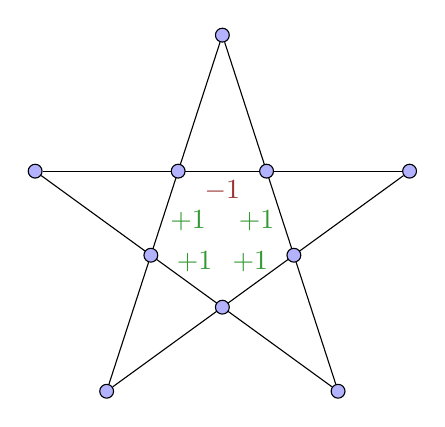
\begin{tikzpicture}[vertex/.style={circle, thin, fill=blue!30, draw, inner sep=0, minimum size=5pt}]
        \foreach \c [evaluate=\c as \ang using {18 + 72*\c}] in {0, 1, 2, 3, 4} {
          \node [vertex] (\c) at (\ang:25mm) {};
        }

        \draw [name path=0--2] (0) -- (2);
        \draw [name path=0--3] (0) -- (3);
        \draw [name path=1--3] (1) -- (3);
        \draw [name path=1--4] (1) -- (4);
        \draw [name path=2--4] (2) -- (4);

        \node [vertex] (01) at (intersection of 0--2 and 1--4) {};
        \node [vertex] (04) at (intersection of 0--3 and 1--4) {};
        \node [vertex] (12) at (intersection of 1--3 and 0--2) {};
        \node [vertex] (23) at (intersection of 1--3 and 2--4) {};
        \node [vertex] (34) at (intersection of 0--3 and 2--4) {};
        
        \node [text=red!50!black!80] (label0--2) at ($(01)!0.5!(12) - (0, 0.25)$) {\(-1\)};
        \node [text=green!50!black!80] (label1--4) at ($(01)!0.5!(04) + (-0.3, -0.1)$) {\(+1\)};
        \node [text=green!50!black!80] (label0--3) at ($(04)!0.5!(34) + (-0.1, 0.25)$) {\(+1\)};
        \node [text=green!50!black!80] (label2--4) at ($(23)!0.5!(34) + (+0.1, 0.25)$) {\(+1\)};
        \node [text=green!50!black!80] (label1--3) at ($(12)!0.5!(23) + (+0.3, -0.1)$) {\(+1\)};
      \end{tikzpicture}
    \end{center}
    \caption{The pentagram game as a hypergraph.}
  \end{subfigure}
  \hfill{}
  \begin{subfigure}[t]{0.49\textwidth}
    \begin{center}
      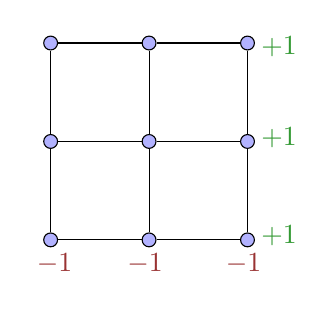
\begin{tikzpicture}[vertex/.style={circle, thin, fill=blue!30, draw, inner sep=0, minimum size=5pt}]
        \node (00) [vertex] at (-1.25, 0) {};
        \node (01) [vertex] at (0,  0) {};
        \node (02) [vertex] at (1.25,  0) {};

        \node (10) [vertex] at (-1.25, -1.25) {};
        \node (11) [vertex] at (0,  -1.25) {};
        \node (12) [vertex] at (1.25,  -1.25) {};

        \node (20) [vertex] at (-1.25, -2.5) {};
        \node (21) [vertex] at (0,  -2.5) {};
        \node (22) [vertex] at (1.25, -2.5) {};
        
        \node (r0) [text=green!50!black!80] at (1.65, -0.05) {\(+1\)};
        \node (r1) [text=green!50!black!80] at (1.65, -1.20) {\(+1\)};
        \node (r2) [text=green!50!black!80] at (1.65, -2.45) {\(+1\)};
        
        \node (c0) [text=red!50!black!80] at (-1.2, -2.8) {\(-1\)};
        \node (c1) [text=red!50!black!80] at (-0.05, -2.8) {\(-1\)};
        \node (c2) [text=red!50!black!80] at (1.2, -2.8) {\(-1\)};

        \path[]
        (00) edge (01) edge (10)
        (01) edge (02) edge (11)
        (02) edge (12)
        
        (10) edge (11) edge (20)
        (11) edge (12) edge (21)
        (12) edge (22)

        (20) edge (21)
        (21) edge (22)
        ;
      \end{tikzpicture}
    \end{center}
    \caption{The magic square game as a hypergraph.}
  \end{subfigure}
  \caption{Examples of hypergraphs representing quantum magic games~\cite{arkhipov2012}.\label{fig:as-graph}}
\end{figure}

We start by defining the notion of \emph{arrangements}, which are
configurations on which Mermin-style games may be
played. \cite{arkhipov2012} defines both unsigned and signed
arrangements. Instead, we shall focus  on \emph{signed}
arrangements, and thus anytime we say ``arrangement'' we mean the
signed version.

\begin{definition}[Arrangement~\cite{arkhipov2012}]\label{def:arrangement}
  An arrangement \(A = (V, E, \ell)\) is a finite connected hypergraph
  with vertex set \(V\) and hyperedge set \(E\), where a hyperedge is
  a nonempty subset of \(V\), such that every vertex \(v \in V\) lies
  in exactly two hyperedges \(e_{0}, e_{1} \in E\) (\emph{connected}
  means that the hypegraph cannot be split into two smaller disjoint
  hypergraphs). The labelling function \(\ell\colon E \to \{+1, -1\}\)
  maps each hyperedge to a sign \(+1\) or \(-1\).
\end{definition}

We will oftenly refer to a hyperedge as a \emph{line}. In
Figure~\ref{fig:as-graph} (a), the lines going through sequences of
four vertices are the hyperedges. Similarly, in
Figure~\ref{fig:as-graph} (b), the horizontal and vertical lines
touching the sequences of three vertices are the hyperedges.  As
already mentioned, arrangements define the configurations on which
games may be played.

\begin{definition}[Classical Realization~\cite{arkhipov2012}]\label{def:classical-re}
  A classical realization of an arrangement \(A = (V, E, \ell)\) is a
  labelling \(c\colon V \to \{+1, -1\}\) that, for every hyperedge
  \(e \in E\), satisfies the property 
  \[
    \prod_{v \in e} c(v) = \ell(e).
  \]
\end{definition}


\begin{tcbexample}{Classical Realization}{class-re}
  Figure~\ref{fig:class-re} depicts an example of a classically
  realizable arrangement. That is, an arrangement for which there exists
  a classical realization.

  \begin{figure}[H]
    \begin{center}
      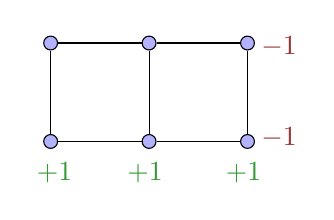
\begin{tikzpicture}[vertex/.style={circle, thin, fill=blue!30, draw, inner sep=0, minimum size=5pt}]
        \node (00) [vertex] at (-1.25, 0) {};
        \node (01) [vertex] at (0,  0) {};
        \node (02) [vertex] at (1.25,  0) {};

        \node (10) [vertex] at (-1.25, -1.25) {};
        \node (11) [vertex] at (0,  -1.25) {};
        \node (12) [vertex] at (1.25,  -1.25) {};

        \node (r0) [text=red!50!black!80] at (1.65, -0.05) {\(-1\)};
        \node (r1) [text=red!50!black!80] at (1.65, -1.20) {\(-1\)};
        
        \node (c0) [text=green!50!black!80] at (-1.2, -1.65) {\(+1\)};
        \node (c1) [text=green!50!black!80] at (-0.05, -1.65) {\(+1\)};
        \node (c2) [text=green!50!black!80] at (1.2, -1.65) {\(+1\)};

        \path[]
        (00) edge (01) edge (10)
        (01) edge (02) edge (11)
        (02) edge (12)
        
        (10) edge (11)
        (11) edge (12)
        ;
      \end{tikzpicture}
    \end{center}
    \caption{Example of a classically realizable arrangement.\label{fig:class-re}}
  \end{figure}

    A classical realization \(c\) for this arrangement is
  \begin{align*}
    c(v_{00}) = c(v_{01}) = c(v_{10}) = c(v_{11}) &= +1 \\
    c(v_{02}) = c(v_{12}) &= -1.
  \end{align*}
\end{tcbexample}


\begin{definition}[Quantum Realization~\cite{arkhipov2012}]\label{def:quantum-re}
  A quantum realization of an arrangement \(A = (V, E, \ell)\) is a
  labelling \(q\colon V \to \operatorname{GL}(\mathcal{H})\) is a
  mapping from each vertex to an observable \(M\) on a fixed
  finite-dimensional Hilbert-space \(\mathcal{H}\), such that
  \begin{itemize}
  \item \(M\) is Hermitian and squares to the identity, or
    equivalently, has eigenvalues \(\pm{}1\);
    
  \item For each hyperedge, the observable assigned to its vertices
    pairwise commute and
    
  \item For each hyperedge \(e \in E\), the labelling of its vertices
    satisfies the property
    \[
      \prod_{v \in e} q(v) = \ell(e) I.
    \]
  \end{itemize}
\end{definition}

A classical realization is simply a quantum realization in which
\(\mathcal{H} = \mathbb{R}\). As such, every classically realizable
arrangement is quantumly realizable. An example of quantum realization
was given in Section~\ref{sec:quantum-sol} for the magic square game.
Any arrangement that is quantumly realizable with observables that all
mutually commute, then it is also classically
realizable~\cite[Proposition 8]{arkhipov2012}. The proof follows by
the simultaneous diagonalization of the observables, similar to our
proof for Lemma~\ref{lem:product}.

It turns out that the existence of a classical or quantum realization
of an arrangement depends only on whether the number of \(-1\) labels
is odd or even. This is called the \emph{parity} of the arrangement.

\begin{definition}[Parity~\cite{arkhipov2012}]\label{def:parity}
  The parity \(p(\ell)\) of an arrangement \(A = (V, E, \ell)\) is
  \[
    p(\ell) = \prod_{e \in E} \ell(E),
  \]
  which is \(-1\) if there is an odd number of \(-1\) labels, or \(+1\) otherwise.
\end{definition}

If there exists a realization (either classical or quantum) of an
arrangement \(A = (V, E, \ell)\), then it is possible to construct a
realization for \(A' = (V, E, \ell')\) from the realization of
\(A\)~\cite[Propositions 10 and 12]{arkhipov2012}. Furthermore, an
arrangement is classically realizable if, and only if, its parity is
\(+1\)~\cite[Proposition 11]{arkhipov2012}. Despite this fundamental result,
Classically realizable arrangements are not as much interesting as the
quantumly ones. Therefore, the goal is to characterize the gap between
these two worlds. The arrangements that are quantumly realizable, but
are not classically realizable, are called \emph{magic} and are
defined as follows:

\begin{definition}[Magic Arrangement~\cite{arkhipov}]\label{def:magic-arr}
  An arrangement is said magic its parity is \(-1\) and it is
  quantumly realizable.
\end{definition}

The magic square and the pentagram are examples of magic arrangements.
Equipped with all these tools, we now define a generalization of \emph{parity}
pseudo-telepathy games (Mermin-style games):

\printbibliography{}
\end{document}
